% Standard pen-and-paper worksheet preamble, in the form m01 and m02 use.
% Compile with: xelatex -interaction=nonstopmode exercise.tex   (run twice)
%
% 14pt, not 12pt: the sheet is read with a pencil in hand. There are no blanks
% and no ruled answer gaps anywhere on it -- questions are asked in words and
% answered on the back -- so the paper those would have cost goes to the text
% and to the drawings.
\documentclass[a4paper, 14pt]{extarticle}
\usepackage[top=0.75in, bottom=0.7in, left=0.85in, right=0.85in]{geometry}
\usepackage{amsmath}
\usepackage{amssymb}
\usepackage{array}
\usepackage{graphicx}
\usepackage[hidelinks]{hyperref}   % hidelinks, or the print carries colour boxes
\usepackage{tcolorbox}
\usepackage{enumitem}
\usepackage{etoolbox}
\usepackage{tikz}
\usepackage{fontspec}
\usetikzlibrary{calc,decorations,patterns,arrows,decorations.pathmorphing,positioning}
\definecolor{pltblue}{HTML}{1F77B4}

% Body face: Charter, and the four ways to get it. XCharter *is* Charter and
% ships with a full TeX Live, so it is asked for first and by file -- a CI
% runner answers yes to \IfFontExistsTF{Charter}, then cannot typeset it, which
% is how these sheets stopped building there.
\IfFontExistsTF{XCharter-Roman.otf}{
  \setmainfont{XCharter}[
    Extension      = .otf,
    UprightFont    = *-Roman,
    BoldFont       = *-Bold,
    ItalicFont     = *-Italic,
    BoldItalicFont = *-BoldItalic]
}{
  \IfFontExistsTF{Charter}{\setmainfont{Charter}}{
    \IfFontExistsTF{Iowan Old Style}{\setmainfont{Iowan Old Style}}{
      \IfFontExistsTF{Georgia}{\setmainfont{Georgia}}{}}}}

% Handwriting face, resolved once into \ppfont. Used for a heading or two (the
% answer key's "Answers"), not for the body and not for the drawings: the
% figures are read closely and want the text face.
%
% Naming a font that is not installed is a hard error, not a fallback, which is
% why this is a chain and not a line: seven sheets used to name one outright and
% stopped building the day it was uninstalled. Write \ppfont, never
% \fontspec{<a name>}. Excalifont is vendored in tools/fonts/ and installed by
% CI, so it is the one face that is always present.
\newcommand{\ppfont}{}
\IfFontExistsTF{Pretty Neat}{\renewcommand{\ppfont}{\fontspec{Pretty Neat}}}{
  \IfFontExistsTF{Humor Sans}{\renewcommand{\ppfont}{\fontspec{Humor Sans}}}{
    \IfFontExistsTF{Excalifont}{\renewcommand{\ppfont}{\fontspec{Excalifont}}}{
      \renewcommand{\ppfont}{}}}}

\setlength{\parindent}{0pt}
\setlength{\parskip}{0.38em}
\setlength{\emergencystretch}{1.2em}
\raggedbottom

% Break the page unless #1 of it is left.
%
% This is needspace's glue trick, written out because needspace.sty lives in
% texlive-latex-extra and not in a BasicTeX install. Do NOT rewrite it as a test
% on \pagegoal minus \pagetotal: the page builder has not necessarily run when
% the macro expands, so those numbers can still be the previous page's, the test
% says "no room" on a page that is empty, and the \newpage throws that page
% away. m02 shipped a blank page 3 that way, and it is invisible in the source.
\newcommand{\needroom}[1]{%
  \par
  \begingroup
    \setlength{\dimen0}{#1}%
    \vskip 0pt plus \dimen0
    \penalty -100%
    \vskip 0pt plus -\dimen0
  \endgroup}

% A part heading. The sheet has no title: it opens on Part 1. The heading
% carries the break test, because a heading printed at the foot of a page with
% nothing under it is worse than a short page.
\newcommand{\parthead}[2]{%
  \needroom{6\baselineskip}%
  \partheadhere{#1}{#2}}

% The same heading with no break test, for one already inside a minipage --
% \newpage means nothing in there.
\newcommand{\partheadhere}[2]{%
  \vspace{0.5em}
  {\large\bfseries Part #1 --- #2}\par
  \vspace{-0.4em}\rule{\textwidth}{0.8pt}\par
  \vspace{0.1em}}

% Centred fixed-width cell, for tables the student writes into.
\newcolumntype{C}[1]{>{\centering\arraybackslash}p{#1}}

% The lab the sheet hands off to, if it has one. Both the QR code and the
% printed address are the course's own short link, never the notebook's: paper
% outlives any one upload, so re-uploading a lab is a line on the server
% (/etc/caddy/Caddyfile, block go.skojaku.com) and not a reprint.
%
%   uvx --from segno segno --output=mNNlab-qr.png --scale=20 --border=4 \
%       --error=m "https://go.skojaku.com/mNNlab"
%
% --border=4 is the quiet zone the QR spec asks for and is not optional: at
% --border=1 some codes run to the edge of the PNG and OpenCV reads nothing.
\newcommand{\molablink}{https://go.skojaku.com/mNNlab}
\newcommand{\molaburl}{\href{\molablink}{\texttt{go.skojaku.com/mNNlab}}}

% xkcd-style hand-drawn line decoration.
% WARNING: applying [xkcd] to many nodes can throw "Dimension too large".
% Use it on a handful of \draw lines only, never on every node.
\makeatletter
\pgfset{
  /pgf/decoration/randomness/.initial=2,
  /pgf/decoration/wavelength/.initial=100
}
\pgfdeclaredecoration{sketch}{init}{
  \state{init}[width=0pt,next state=draw,persistent precomputation={
    \pgfmathsetmacro\pgf@lib@dec@sketch@t0
  }]{}
  \state{draw}[width=\pgfdecorationsegmentlength,
  auto corner on length=\pgfdecorationsegmentlength,
  persistent precomputation={
    \pgfmathsetmacro\pgf@lib@dec@sketch@t{mod(\pgf@lib@dec@sketch@t+pow(\pgfkeysvalueof{/pgf/decoration/randomness},rand),\pgfkeysvalueof{/pgf/decoration/wavelength})}
  }]{
    \pgfmathparse{sin(2*\pgf@lib@dec@sketch@t*pi/\pgfkeysvalueof{/pgf/decoration/wavelength} r)}
    \pgfpathlineto{\pgfqpoint{\pgfdecorationsegmentlength}{\pgfmathresult\pgfdecorationsegmentamplitude}}
  }
  \state{final}{}
}
\tikzset{xkcd/.style={decorate,decoration={sketch,segment length=0.5pt,amplitude=0.5pt}}}
\makeatother

% Degree box beside a student in Part 2's drawing, written into in Part 3.
\tikzset{
  stu/.style={draw, circle, minimum size=0.85cm, inner sep=0pt, font=\bfseries},
  dbox/.style={draw, minimum size=0.6cm, inner sep=0pt},
  pal/.style={draw, circle, minimum size=0.9cm, inner sep=0pt},
}

% A five-member study group on a pentagon. #1 = the friendships.
\newcommand{\pentagroup}[1]{%
\begin{tikzpicture}[thick]
  \node[pal] (1) at (90:1.9) {1};
  \node[pal] (2) at (18:1.9) {2};
  \node[pal] (3) at (-54:1.9) {3};
  \node[pal] (4) at (-126:1.9) {4};
  \node[pal] (5) at (162:1.9) {5};
  \foreach \a/\b in {#1} \draw (\a) -- (\b);
\end{tikzpicture}}

\begin{document}

\parthead{1}{How imperfect can a group be?}

Here are two study groups of five. In neither group is everybody friends with
everybody. Each group has seven friendships.

\begin{center}
\begin{tabular}{c@{\hspace{2.2cm}}c}
\pentagroup{1/2,1/5,2/3,2/5,3/4,3/5,4/5} &
\pentagroup{1/2,2/3,4/5,5/1,1/3,5/3,5/2} \\[0.3em]
the Monday group & the Friday group
\end{tabular}
\end{center}

{\bf Question 1}: Without counting anything, which of the two looks more like a
real group to you? Say why in one sentence.

{\bf Question 2}: Work out four numbers for each group and write them in the
table.

\begin{center}
\renewcommand{\arraystretch}{1.25}
\begin{tabular}{|p{2.3cm}|C{3cm}|C{3cm}|C{3cm}|C{3cm}|}
\hline
& the fewest friends any member has
& the most members any one person is \emph{not} friends with
& friendships, out of the 10 possible
& the most steps between two members \\
\hline
name & & & & \\[0.9cm]
\hline
Monday & & & & \\[0.9cm]
\hline
Friday & & & & \\[0.9cm]
\hline
\end{tabular}
\end{center}

Each column is one of the four definitions from the lecture: $k$-core,
$k$-plex, $\rho$-dense and $n$-clique. Write the right name in the ``name'' row.

\needroom{4\baselineskip}%
{\bf Question 3}: Which columns say the Monday group and the Friday group are
equally good groups?

Which columns tell them apart?

Look at person 4 in the Friday group. Is person 4 part of that group? Which
column would you use to decide? Does your neighbour pick the same one?

\parthead{2}{Two teams}

You teach a lab section of eight students, A to H. The lines are the ten
friendships between them. You want to split the section into two teams and
keep friends together. The boxes are for Part 3; leave them empty for now.

\begin{center}
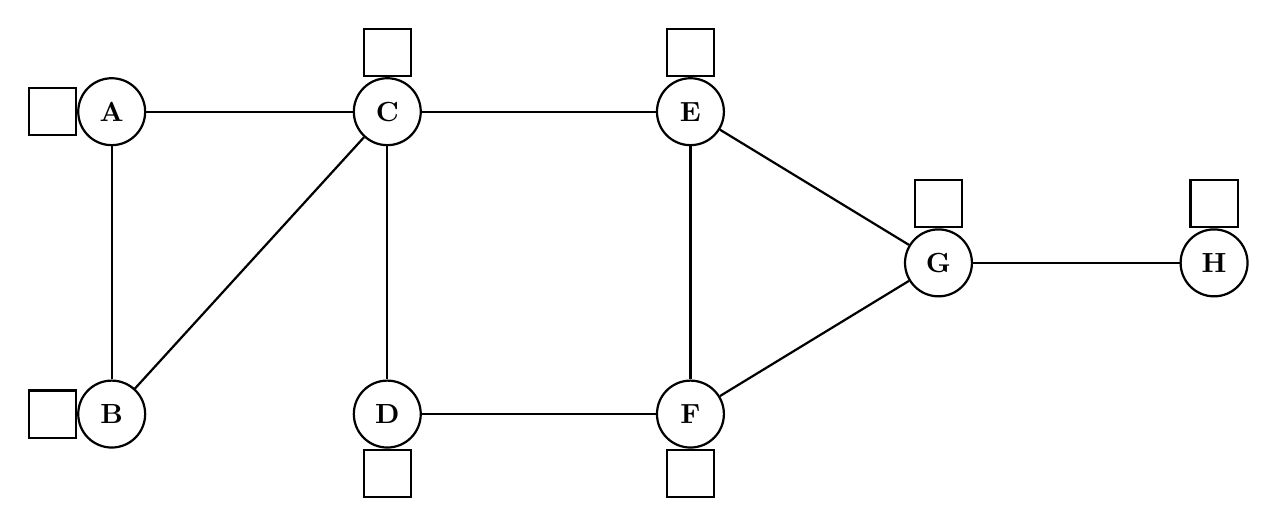
\begin{tikzpicture}[thick, x=1.75cm, y=1.6cm]
  \node[stu, label={[dbox]180:{}}] (A) at (0,2.4) {A};
  \node[stu, label={[dbox]180:{}}] (B) at (0,0) {B};
  \node[stu, label={[dbox]90:{}}]  (C) at (2,2.4) {C};
  \node[stu, label={[dbox]-90:{}}] (D) at (2,0) {D};
  \node[stu, label={[dbox]90:{}}]  (E) at (4.2,2.4) {E};
  \node[stu, label={[dbox]-90:{}}] (F) at (4.2,0) {F};
  \node[stu, label={[dbox]90:{}}]  (G) at (6,1.2) {G};
  \node[stu, label={[dbox]90:{}}]  (H) at (8,1.2) {H};
  \foreach \a/\b in {A/B,A/C,B/C,C/D,C/E,D/F,E/F,E/G,F/G,G/H}
    \draw (\a) -- (\b);
\end{tikzpicture}
\end{center}

{\bf Question 4}: Draw one line on the drawing that splits the eight students
into two teams. Cross as few friendships as you can.

How many friendships does your line cross?

\needroom{3\baselineskip}%
{\bf Question 5}: Compare with your neighbour. Is there a line that crosses
even fewer friendships?

Would you really use that line to make two teams? Why?

\needroom{8\baselineskip}%
{\bf Question 6}: Here are two ways to split the section.

\quad Split X: \ H alone, and the other seven together.

\quad Split Y: \ A, B, C, D in one team, and E, F, G, H in the other.

For each split, count the friendships it crosses. Then work out the ratio cut
from the lecture:
\[
\text{ratio cut} \;=\; \frac{\text{friendships crossed}}
{(\text{people in team 1}) \times (\text{people in team 2})}
\]
A lower ratio cut is a better split. Which split wins now? What did dividing by
the two team sizes change?

\newpage
\parthead{3}{More than chance}

Play the game from the lecture. Every friendship is a string with a ball on
each end, so the ten friendships in Part 2 make twenty balls. A student with
three friends holds three balls. Paint each ball in the colour of its owner's
team.

{\bf Question 7}: In each box on the drawing in Part 2, write how many friends
that student has.

\needroom{12\baselineskip}%
{\bf Question 8}: Score four ways to make teams. For each row:

\begin{itemize}[leftmargin=1.5em, itemsep=0pt, topsep=2pt]
\item \emph{observed}: friendships inside a team, divided by 10.
\item \emph{chance}: for each colour, take (balls of that colour $\div$ 20),
  square it, and add these up over the colours.
\item $Q$ = observed $-$ chance.
\end{itemize}

\begin{center}
\renewcommand{\arraystretch}{1.25}
\begin{tabular}{|>{\raggedright\arraybackslash}p{4.0cm}|C{2.5cm}|C{2.4cm}|C{2cm}|C{1.8cm}|C{1.3cm}|}
\hline
teams & friendships inside a team & balls of each colour & observed & chance & $Q$ \\
\hline
everybody in one team & & & & & \\[1.1cm]
\hline
Split X: \{H\}, \{the rest\} & & & & & \\[1.1cm]
\hline
Split Y: \{A,B,C,D\}, \{E,F,G,H\} & & & & & \\[1.1cm]
\hline
\{A,B,C,D\}, \{E,F,G\}, \{H\} & & & & & \\[1.1cm]
\hline
\end{tabular}
\end{center}

\needroom{4\baselineskip}%
{\bf Question 9}: Which row has the highest $Q$?

Split X crossed the fewest friendships in Part 2. What does $Q$ say about it?

The ratio cut in Question 6 had to be told ``two teams''. Did anybody tell $Q$
how many teams to make?

\needroom{3\baselineskip}%
{\bf Question 10}: Without calculating: put every student in a team of their
own, eight teams of one. What is \emph{observed}? Is $Q$ positive or negative?
Why?

\end{document}
